\documentclass[t,aspectratio=169]{beamer}
%\usetheme{Berkeley}
\usepackage{graphicx}
\usepackage{amsmath}
\usepackage[american]{circuitikz}

\title{Clase 13}
\subtitle{El transistor bipolar}
\author{Dr.-Ing. Juan José Montero Rodríguez}
\subject{Elementos Activos}
\institute{Escuela de Ingeniería Electrónica}
\date{Semestre II-2023}

\begin{document}

\begin{frame}{}
\maketitle
\end{frame}


\section{Fundamentos}
\begin{frame}{El transistor de unión bipolar (BJT)}

\begin{columns}
\begin{column}{0.5\textwidth}

\begin{figure}
    \centering
    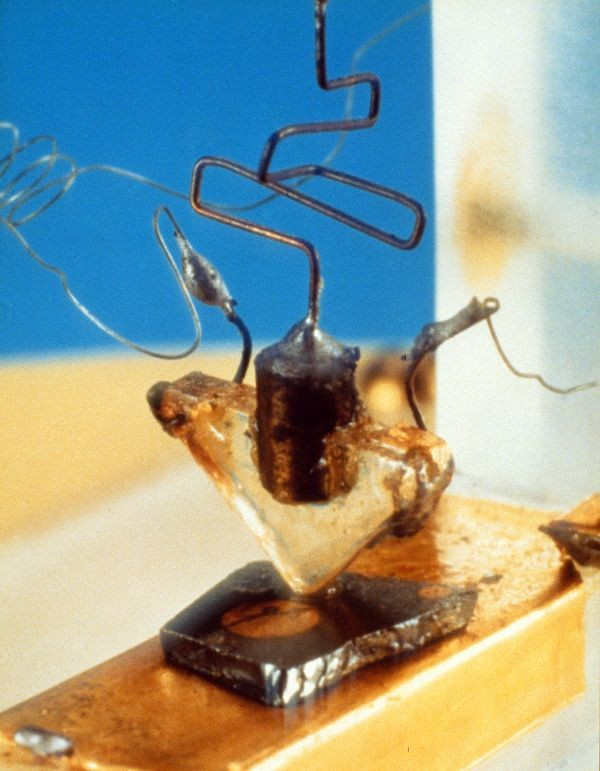
\includegraphics[height=6.5cm]{figures/the_first_transistor.jpg}
\end{figure}

\end{column}
\begin{column}{0.5\textwidth}
    \textbf{BJT: Bipolar Junction Transistor}

    Inventado en Laboratorios Bell, 1947

    \vspace{5mm}
    Coinventores:
    
    Dr. William Shockley;
    
    Dr. John Bardeen;
    
    Dr. Walter H. Brattain.

    \begin{figure}
        \centering
        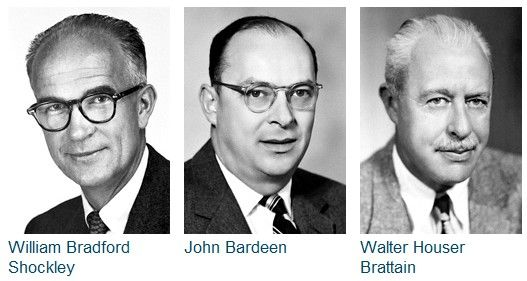
\includegraphics[width=\textwidth]{figures/the_first_transistor_2.jpg}
    \end{figure}

\end{column}
\end{columns}

\end{frame}


\begin{frame}{Construcción de un transistor BJT}
\begin{columns}
\begin{column}{0.5\textwidth}

El transistor de unión bipolar está formado por tres regiones de silicio:

\begin{itemize}
    \item Colector
    \item Base
    \item Emisor
\end{itemize}

En un transistor BJT típico:

\begin{itemize}
    \item El emisor tiene un dopado más alto que el colector.
    \item La base es mucho más delgada que las otras regiones.
    \item Las terminales del emisor y el colector NO son intercambiables.
\end{itemize}

\end{column}
\begin{column}{0.5\textwidth}

    \begin{figure}
        \centering
        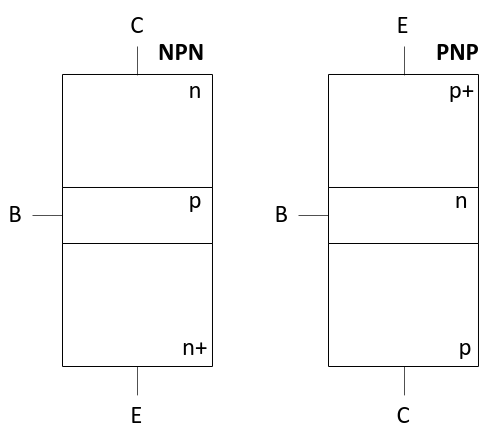
\includegraphics[width=\textwidth]{figures/construccion_transistor.png}
    \end{figure}

\end{column}
\end{columns}

\end{frame}


\begin{frame}{Símbolo de un transistor BJT}
\begin{columns}
\begin{column}{0.5\textwidth}

Los símbolos de los transistores son:

\begin{figure}
    \centering
    \begin{circuitikz}
        \draw (0,0) node[npn](npn1){};
        \draw (0,1.5) node[above](){\textbf{NPN}};
        \draw (npn1.collector) node[above]{C};
        \draw (npn1.base) node[left]{B};
        \draw (npn1.emitter) node[below]{E};
        \draw (3,0) node[pnp](pnp1){};
        \draw (3,1.5) node[above](){\textbf{PNP}};
        \draw (pnp1.collector) node[below]{C};
        \draw (pnp1.base) node[left]{B};
        \draw (pnp1.emitter) node[above]{E};
    \end{circuitikz}
\end{figure}

\begin{itemize}
    \item La flecha del símbolo representa un diodo entre la base y el emisor.
    \item La corriente en el transistor siempre va en la dirección de la flecha.
\end{itemize}

\end{column}
\begin{column}{0.5\textwidth}

    \begin{figure}
        \centering
        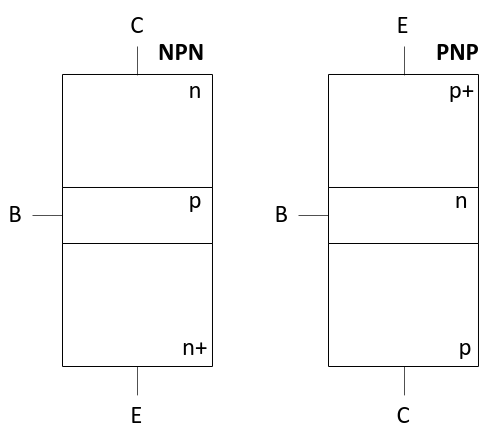
\includegraphics[width=\textwidth]{figures/construccion_transistor.png}
    \end{figure}

\end{column}
\end{columns}

\end{frame}


\section{Funcionamiento}
\begin{frame}{Funcionamiento del transistor BJT}

Un transistor convierte la \textbf{tensión de entrada} en una \textbf{corriente de salida}.

\begin{columns}
\begin{column}{0.3\textwidth}

\begin{figure}
    \centering
    \begin{circuitikz}[scale=0.8]
        \draw (0,0) node[npn](npn1){};
        \draw (-2,0) -- (npn1.base);
        \draw (-2,0) to [V,l=$V_{in}$] (-2,-2);
        \draw (-2,-2) node[ground]{};
        \draw (0,-2) node[ground]{};
        \draw (npn1.emitter) -- (0,-2);
        \draw (0,3) to [R,l=$R_C$] (npn1.collector);
        \draw (0,3) node[vcc]{$V_{CC}$};
        \draw[->] (0.25,1) -- (0.25,0.5);
        \draw (0.25,0.75) node[right]{$I_{out}$};
    \end{circuitikz}
\end{figure}

\end{column}
\begin{column}{0.7\textwidth}

La corriente de salida $I_{out}$ NO depende del valor de la resistencia $R_C$.
%
\[ I_{out} = I_C \]
%
\[ V_{in} = V_{BE} \]
%
El funcionamiento del transistor se describe por medio de la \textbf{Ecuación de Shockley}:
%
\[ I_C = I_S \cdot ( e^{V_{BE}/V_t} - 1 ) \]
%
La ecuación es válida sólo si el diodo B-E está encendido:
%
\[ V_{BE} > 0.7\ V \]
\end{column}
\end{columns}
\end{frame}


\begin{frame}{Región de operación activa directa}
\begin{columns}
\begin{column}{0.5\textwidth}

El transistor bipolar está compuesto por dos uniones de tipo P-N conectadas de la siguiente manera:

\begin{figure}
    \centering
    \scalebox{1}{\begin{circuitikz}
        \draw (0,0) to[D,l=$D_{BE}$,-o] (0,-2);
        \draw (0,0) to[D,l_=$D_{BC}$,-o] (0,2);
        \draw (0,0) to[short,-o] (-1,0);
        \draw (0,-2) node[below]{E};
        \draw (0,2) node[above]{C};
        \draw (-1,0) node[left]{B};
    \end{circuitikz}}
\end{figure}

\end{column}
\begin{column}{0.5\textwidth}

Para que la corriente de colector $I_C$ sea función de la tensión de entrada $V_{BE}$, es necesario que se cumplan las siguientes dos condiciones:
%
\[ V_{BE} > 0.7\ V \]
%
\[ V_{BC} < 0 \]
%
En otras palabras:

\begin{itemize}
    \item El diodo B-E debe estar encendido.
    \item El diodo B-C debe estar apagado.
\end{itemize}
%
\[ \boxed{V_{CE} > V_{BE}} \]

\end{column}
\end{columns}
\end{frame}


\begin{frame}{Funcionamiento en la región activa directa}
\begin{columns}
\begin{column}{0.5\textwidth}

El funcionamiento del transistor BJT NPN se explica en la siguiente secuencia:

\vspace{5mm}
\begin{itemize}
    \item Se inyectan huecos en la base.
    \item Los huecos fluyen de B$\rightarrow{}$E.
    \item Los electrones fluyen de E$\rightarrow{}$B.
    \item Los electrones que ingresan a la base entran rápidamente en la región de agotamiento B-C.
    \item El colector ``recolecta" los electrones, electrones fluyen de B$\rightarrow{}$C.
\end{itemize}

\end{column}
\begin{column}{0.5\textwidth}

\begin{figure}
    \centering
    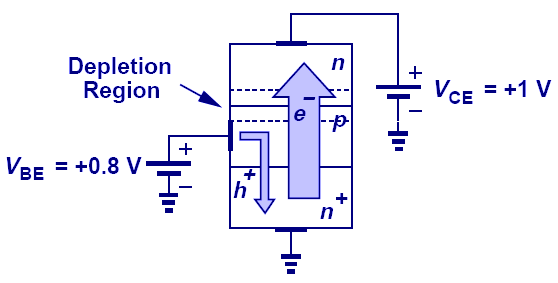
\includegraphics[width=\textwidth]{figures/transistor_funcionamiento.png}
\end{figure}

Para el transistor BJT PNP se sigue el mismo análisis, inyectando electrones en la base.

\end{column}
\end{columns}
\end{frame}


\begin{frame}{Acción del colector}

\begin{itemize}
    \item Una unión PN en reversa tiene un campo eléctrico en la zona de agotamiento.
    \item Si se inyectan portadores minoritarios (electrones) en la región p, el campo eléctrico atrae los electrones hacia la región n.
    \item La terminal n ``recolecta" los electrones inyectados.
\end{itemize}

\begin{figure}
    \centering
    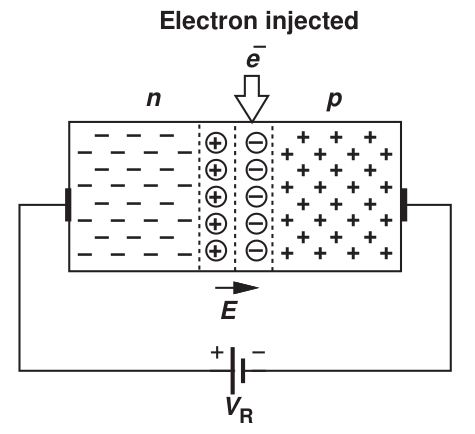
\includegraphics[width=0.4\textwidth]{figures/transistor_accion_colector.png}
\end{figure}
    
\end{frame}


\section{Curvas características}
\begin{frame}{Curva de transferencia}

\begin{columns}
\begin{column}{0.5\textwidth}

La curva de transferencia se mide al dejar $V_{CE}$ constante y modificar $V_{BE}$.

\begin{figure}
    \centering
    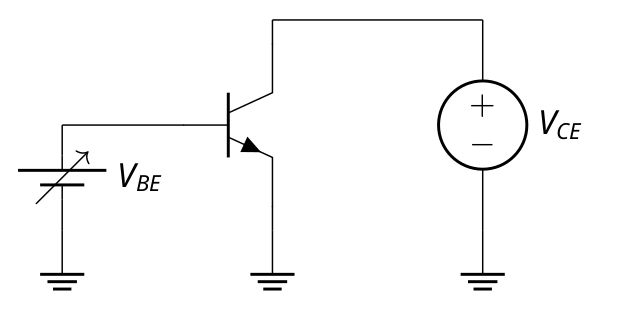
\includegraphics[width=\textwidth]{figures/curva_transferencia_1.png}
\end{figure}
%
\[ I_C = I_S \cdot (e^{V_{BE}/V_t} - 1) \]

\end{column}
\begin{column}{0.5\textwidth}

\begin{figure}
    \centering
    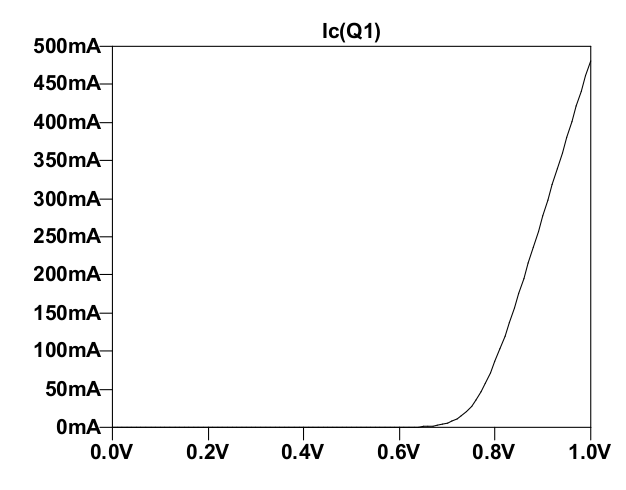
\includegraphics[width=\textwidth]{figures/curva_transferencia_2.png}
\end{figure}

\end{column}
\end{columns}

\end{frame}


\begin{frame}{Curva de salida}

\begin{columns}
\begin{column}{0.5\textwidth}

La curva de salida se mide al dejar $V_{BE}$ constante y modificar $V_{CE}$.

\begin{figure}
    \centering
    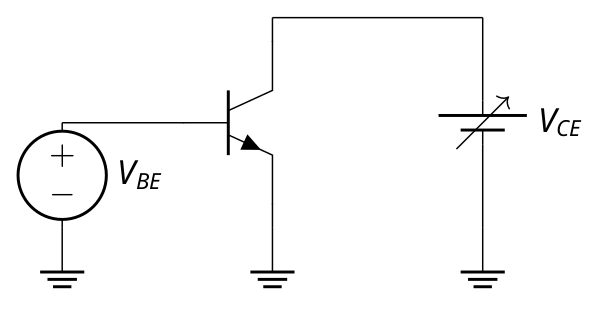
\includegraphics[width=\textwidth]{figures/curva_salida_1.png}
\end{figure}
%
\textbf{Activa directa:} fuente de corriente.

\textbf{Saturación:} corriente no es estable.


\end{column}
\begin{column}{0.5\textwidth}

\begin{figure}
    \centering
    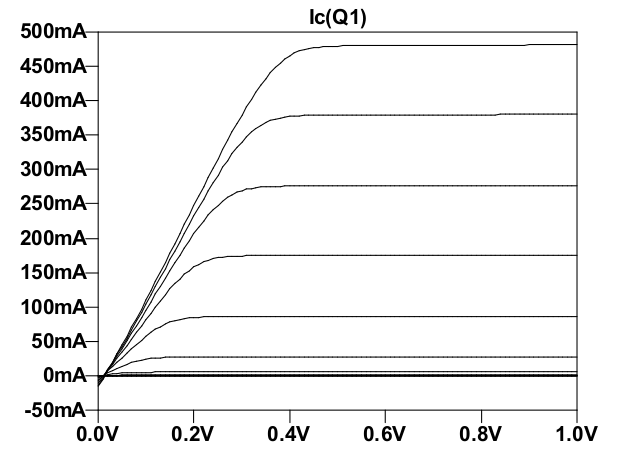
\includegraphics[width=\textwidth]{figures/curva_salida_2.png}
\end{figure}

\end{column}
\end{columns}

\end{frame}


\section{Relaciones de corriente}
\begin{frame}{Fuente de corriente constante}

\begin{itemize}
    \item Idealmente, la corriente de colector $I_C$ no depende de la tensión colector-emisor $V_{CE}$.
    \item Esta propiedad le permite al transistor funcionar como una fuente de corriente constante, cuando la tensión base-emisor $V_{BE}$ es fija.
\end{itemize}

\begin{figure}
    \centering
    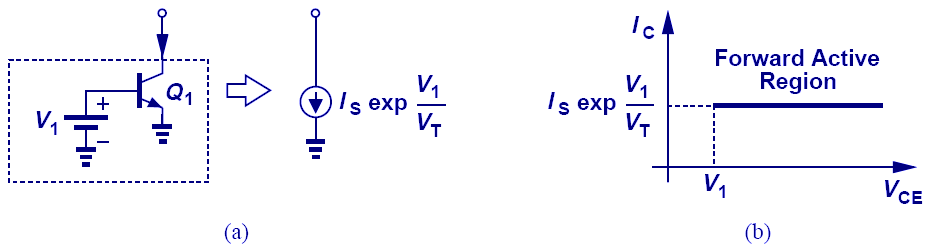
\includegraphics[width=\textwidth]{figures/transistor_como_fuente_corriente.png}
\end{figure}
    
\end{frame}


\begin{frame}{Corriente de colector}

\begin{itemize}
    \item Aplicando la ley de difusión, se puede determinar el flujo de carga desde la base hasta el colector.
    \item La ecuación muestra que la corriente $I_C$ del transistor está controlada por la tensión $V_{BE}$, haciéndolo buen candidato como amplificador.
\end{itemize}

\begin{columns}
\begin{column}{0.5\textwidth}

\[ I_C = I_S \cdot (e^{V_{BE}/V_t} - 1) \]

\[ I_C = \dfrac{A_E q D_n n_i^2}{N_E W_B} \cdot (e^{V_{BE}/V_t} - 1) \]

\[ I_S = \dfrac{A_E q D_n n_i^2}{N_E W_B} \]

\end{column}
\begin{column}{0.5\textwidth}

$A_E$: área del emisor

$q$: carga del electrón

$D_n$: coeficiente de difusión de electrones

$n_i^2$: concentración intrínseca de electrones

$N_E$: concentración de dopado del emisor

$W_B$: ancho de la base

$V_t$: tensión térmica 25.85 mV a T=300 K.

$I_S$: corriente de saturación reversa de B-E.

\end{column}
\end{columns}

\end{frame}


\begin{frame}{Corriente de base y corriente de colector}

Si se conoce la corriente de colector, se puede determinar la corriente en las otras terminales.

\begin{columns}
\begin{column}{0.5\textwidth}
    \begin{itemize}
        \item Se define la ganancia de corriente de emisor común:
        \[ \beta = \dfrac{I_C}{I_B} \]
        \item Se define la ganancia de corriente de base común:
        \[ \alpha = \dfrac{I_C}{I_E} \]
    \end{itemize}
\end{column}
\begin{column}{0.5\textwidth}

\[ I_C = \beta I_B \]
%
\[ I_E = I_C + I_B \]
%
\[ I_E = (\beta + 1) I_B \]

\vspace{5mm}
\[ \alpha = \dfrac{\beta}{\beta + 1} \]
%
\[ \beta = \dfrac{\alpha}{1 - \alpha} \]
\end{column}
\end{columns}

\end{frame}


\section{Ejemplos}
\begin{frame}{Ejemplo 1: Corrientes en el transistor NPN}

El transistor NPN de la figura se encuentra a temperatura ambiente $T=300\ K$ y presenta un parámetro $I_S = 4 \times 10^{-16}\ A$. La ganancia de corriente es $\beta = 100$.

\begin{enumerate}
    \item Determine la corriente de colector, la corriente de emisor y la corriente de base.
    \item Calcule la tensión en el colector.
    \item Determine la máxima resistencia de colector permitida para que Q1 permanezca en activa directa.
\end{enumerate}

\begin{figure}
    \centering
    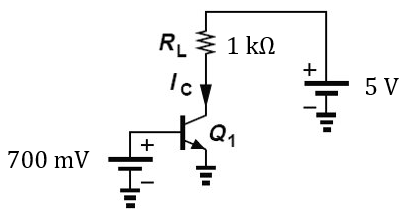
\includegraphics[width=6cm]{figures/ejemplo_1.png}
\end{figure}

\end{frame}


\begin{frame}{Solución 1: Corrientes en el transistor NPN}

\begin{columns}
\begin{column}{0.5\textwidth}

\begin{figure}
    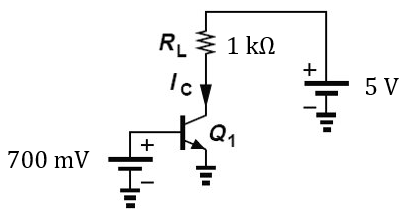
\includegraphics[width=6cm]{figures/ejemplo_1.png}
\end{figure}

\end{column}
\begin{column}{0.5\textwidth}

1. La corriente de colector:
%
\begin{align*}
I_C &= I_S \cdot e^{\dfrac{V_{BE}}{V_t}} \\
I_C &= (4\times{}10^{-16}\ A) \cdot e^{(700\ mV / 26\ mV)} \\
I_C &= 197\ \mu A \\
\end{align*}
%
2. La tensión en el colector:
%
\begin{align*}
V_C &= V_{CC} - I_C R_L \\
V_C &= 5\ V - (197\ \mu A) (1\ k\Omega) \\
V_C &= 4.8\ V
\end{align*}

\end{column}
\end{columns}

\end{frame}


\begin{frame}{Solución 1: Corrientes en el transistor NPN}

\begin{columns}
\begin{column}{0.5\textwidth}

\begin{figure}
    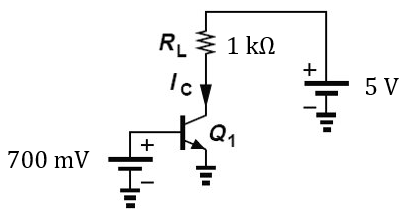
\includegraphics[width=6cm]{figures/ejemplo_1.png}
\end{figure}

\end{column}
\begin{column}{0.5\textwidth}

3. La máxima resistencia de colector permitida:
%
\begin{align*}
V_B &< V_{CC} - I_C R_L \\
I_C R_L &< V_{CC} - V_B \\
R_L &< \dfrac{V_{CC} - V_B}{I_C} \\
R_L &< \dfrac{5\ V - 0.7\ V}{197\ \mu A} \\
R_L &< 21.8\ k\Omega \\
\end{align*}

\end{column}
\end{columns}
\end{frame}


\begin{frame}{Ejemplo 2: Corriente en un transistor PNP}

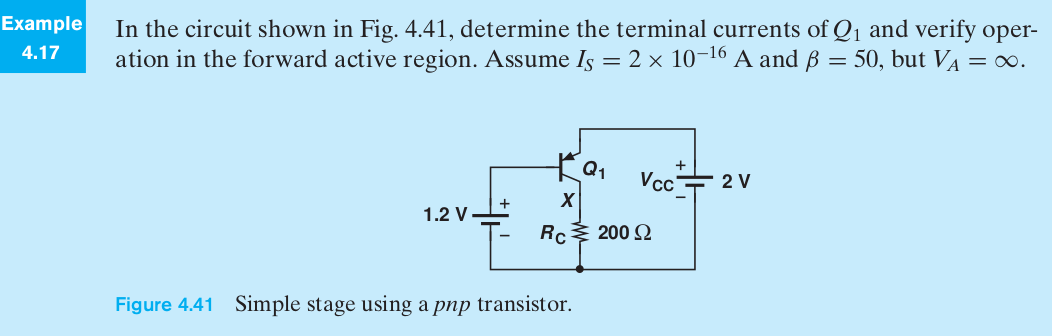
\includegraphics[width=\textwidth]{figures/ejemplo_2.png}

\end{frame}


\begin{frame}{Solución 2: Corriente en un transistor PNP}

\begin{columns}
\begin{column}{0.5\textwidth}

\begin{figure}
    \centering
    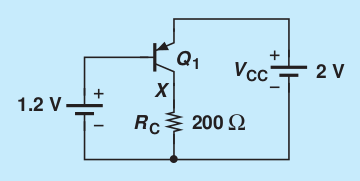
\includegraphics[width=0.8\textwidth]{figures/ejemplo_2b.png}
\end{figure}
%
\[ V_B = 1.2\ V \]
%
\[ V_E = 2\ V \]
%
\[ V_{EB} = V_E - V_B \]
%
\[ V_{EB} = 2\ V - 1.2\ V \]
%
\[ V_{EB} = 0.8\ V \]

\end{column}
\begin{column}{0.5\textwidth}

La corriente de colector:
%
\begin{align*}
I_C &= I_S \cdot e^{V_{EB}/V_t} \\
I_C &= (2\times{}10^{-16}\ A) \cdot e^{0.8/0.026} \\
I_C &= 4.613\ mA
\end{align*}
%
La tensión en el colector:
%
\[ V_C = I_C R_C = (4.613\ mA)(200\ \Omega) \]
%
\[ V_C = 0.923\ V \]

Como $V_C < V_B$, el diodo C-B está apagado. Por lo tanto, sí está en activa directa.

\end{column}
\end{columns}
    
\end{frame}


\section{Circuitos integrados}
\begin{frame}{Construcción de transistores en circuitos integrados}

Los circuitos integrados se construyen sobre obleas de silicio.

\begin{columns}
\begin{column}{0.5\textwidth}

\begin{figure}
    \centering
    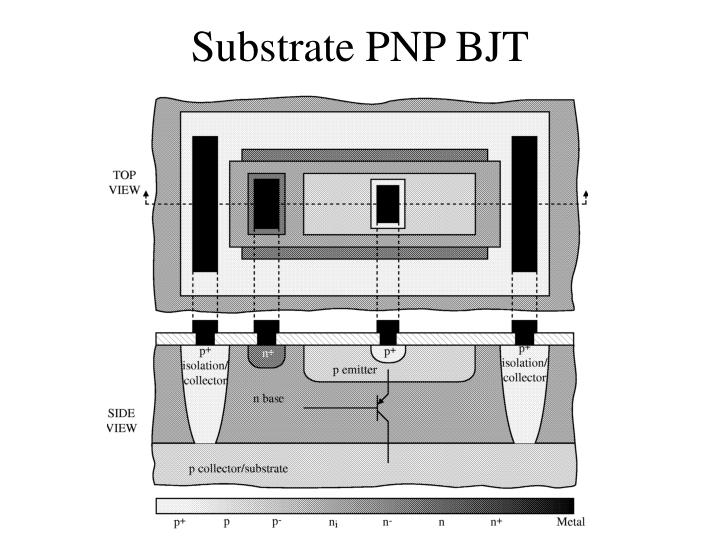
\includegraphics[width=\textwidth]{figures/vertical_pnp_bjt.jpg}
\end{figure}

\end{column}
\begin{column}{0.5\textwidth}

\begin{figure}
    \centering
    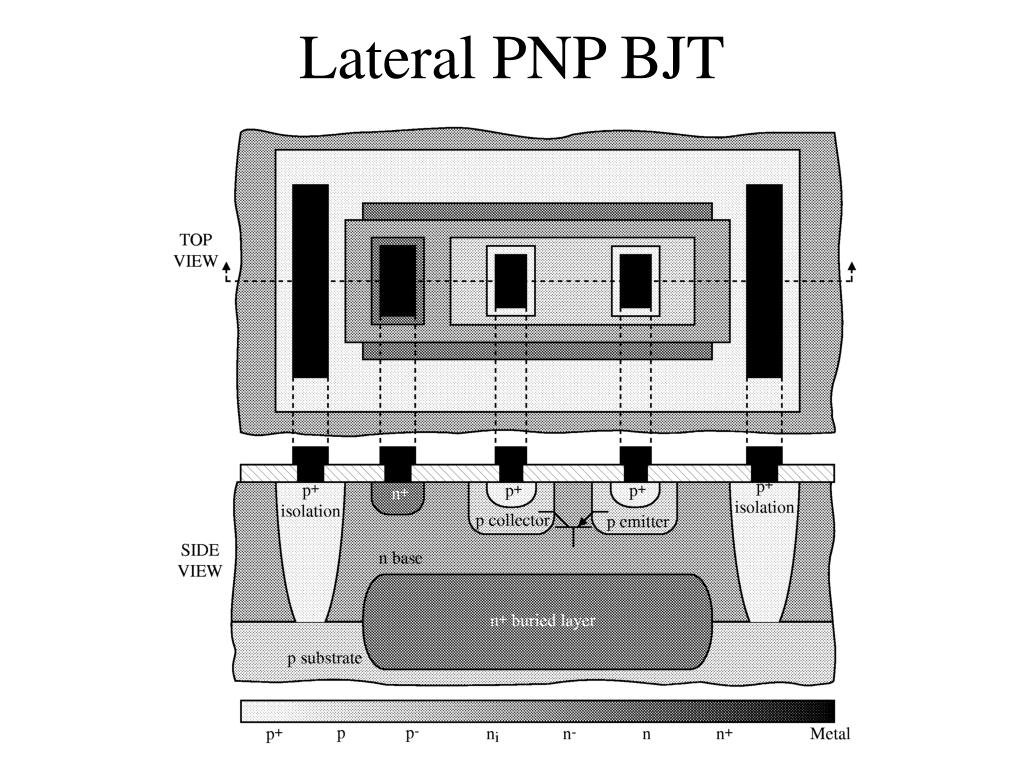
\includegraphics[width=\textwidth]{figures/lateral_pnp_bjt.jpg}
\end{figure}

\end{column}
\end{columns}

\end{frame}


\section{Referencias}
\begin{frame}{Lecturas recomendadas}

\begin{itemize}
    \item Boylestad, R. y Nashelsky, L. (2009). Electrónica: Teoría de Circuitos y Dispositivos Electrónicos. Capítulo 3: Transistores de unión bipolar, pp. 131-138, Pearson Educación, México.
    \item Razavi, B. (2013). Fundamentals of Microelectronics, 2nd edition. Chapter 4: Physics of Bipolar Transistors, pp. 122-133, Wiley, Los Angeles, California.
\end{itemize}
    
\end{frame}

\end{document}
